\section{Grundlagen}
\label{sec:grundlagen}

\subsection{Neuronale Netze}
\label{sec:neuronale-netze}

Neuronale Netze sind eine Modellklasse, welche zur L\"osung des
bereits ausf\"uhrlich
in~\cite{statistical_learning} beschriebenen Problems des statistischen
Lernens eingesetzt werden k\"onnen.
In dieser Problemsituation wird angenommen, dass sich der Zusammenhang zwischen
beobachtbaren Pr\"adiktorvariablen $X_1, ..., X_p$, welche sich durch
einen Vektor $X = (X_1, ..., X_p)$ zusammenfassen lassen, und einer
Zielvariable $Y$ durch eine Funktion $f^*$ mit $Y = f^*(X) + \epsilon$
modellieren l\"asst. Hierbei kann $\epsilon$ als eine zuf\"allige
St\"orgr\"o{\ss}e angesehen werden, die hier im weiteren Verlauf aber
keine wichtige Rolle spielt.
Das Ziel von Neuronalen Netzen ist es, die unbekannte Funktion $f^*$
zu approximieren.

Die folgenden Erkl\"arungen zum Aufbau und zum Training neuronaler Netze
st\"utzen sich wesentlich auf~\cite{Goodfellow-et-al-2016} und sind hier
auf das grundlegendste reduziert worden.
Obwohl es der Name \textit{neuronale} Netze suggeriert, wird auch hier
genau wie in~\cite{Goodfellow-et-al-2016} ebenfalls auf jegliche
biologische Motivation verzichtet, damit nicht der f\"alschliche Eindruck
entstehen kann, dass es sich bei neuronalen Netzen um Modelle von echten
biologischen Gehirnen handeln k\"onnte.
Das Ziel von neuronalen Netzen ist es viel eher, unbekannte Funktionen
anhand von Trainingsdaten zu approximieren und die Ergebnisse dann auf
ungesehene Daten zu generalisieren.

\subsubsection{Aufbau}
\label{sec:aufbau}

Wie in~\ref{sec:neuronale-netze} angedeutet, definiert ein neuronales Netz
also eine Abbildung $f$, welche den Zusammenhang zwischen einer Eingabe $X$
und einer Ausgabe $Y$ approximieren soll.
Eine Hauptcharakteristik von neuronalen Netzen ist es, dass die Funktion $f$
durch die Verkettung weiterer Funktionen gebildet wird.
Ist ein neuronales Netz beispielsweise durch
$f(x) = f^{(3)}(f^{(2)}(f^{(1)}(x)))$ gegeben, so setzt es sich aus der
Verkettung der einzelnen Funktionen $f^{(1)}$, $f^{(2)}$ und
$f^{(3)}$ zusammen. Wie genau diese Funktionen aussehen k\"onnen, soll an dieser
Stelle bewusst ersteinmal offen bleiben.

Solche Ketten von Funktionen k\"onnen gut durch
azyklische Graphen beschrieben werden. Hierbei wird jedes Zwischenergebnis
durch einen Knoten repr\"asentiert, jede Kante zwischen zwei Knoten beschreibt
die Operation, die von einen Ergebnis zum n\"achsten gef\"uhrt hat.
Der Beispielgraph zu $f(x) = f^{(3)}(f^{(2)}(f^{(1)}(x)))$ ist in
Abbildung~\ref{fig:einfacher-graph} zu sehen.

\begin{figure}[h]
    \centering
    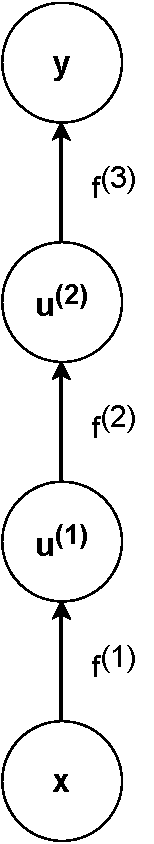
\includegraphics[height=0.3\textheight]{abbildungen/basic_network_graph}
    \caption{Verkettung dreier Funktionen dargestellt als azyklischer Graph.}
    \label{fig:einfacher-graph}
\end{figure}

Im Kontext von neuronalen Netzen wird jede der Funktionen
$f^{(1)}$, $f^{(2)}$ und $f^{(3)}$ auch als eine \textbf{Schicht} im
neuronalen Netz bezeichnet.
Da $f^{(1)}$ und $f^{(2)}$ im Inneren des Netzwerks liegen, bezeichnet man
diese Schichten auch als \textbf{versteckte Schichten}.
Die Gesamtanzahl der Schichten wird als die \textbf{Tiefe} des neuronalen
Netzes bezeichnet.

Zusammenfassend l\"asst sich also sagen, dass sich ein neuronales Netz als
eine Verkettung beliebiger Funktionen auffassen l\"asst, welche auf
eine Eingabegr\"o{\ss}e $X$ angewendet werden.
Wie genau diese Funktionen, also die Schichten des neuronalen Netzes,
aussehen k\"onnen, wird nun im n\"achsten
Abschnitt beschrieben.

\subsubsection{Schichten}

Eine Schicht eines neuronalen Netzes ist eine Funktion $f$, die eine
Eingabe $x \in \mathbb{R}^n$ auf eine Ausgabe $f(x) \in \mathbb{R}^m$
abbildet. H\"aufig hat $f$ dabei die folgende Form:
\begin{equation}
    f(x) = g(Wx + b)
\end{equation}
$W \in \mathbb{R}^{m \times n}$ ist hierbei eine sogenannte Gewichtsmatrix,
die die Eingabe $x$ der Schicht linear transformiert.
$b \in \mathbb{R}^m$ wird auch Bias genannt und wird auf das Ergebnis der
Multiplikation von $W$ mit $x$ addiert.
Die Funktion $g: \mathbb{R}^m \rightarrow \mathbb{R}^m$ hei{\ss}t
Aktivierungsfunktion.

Oftmals ist es so, dass Aktivierungsfunktionen elementweise auf das
Resultat von $Wx + b$ angewendet werden. Hierzu kann man sich eine
Funktion $\Phi: \mathbb{R} \rightarrow \mathbb{R}$ definieren und dann
$g_i(u) = \Phi(u_i), \  i=1,...,m$ setzen. Hierbei beschreibt $g_i$
das $i$-te Element der vektorwertigen Funktion $g$ und $u_i$ das $i$-te
Element des Vektors $Wx + b$.

Die Parameter $W$ und $b$ einer Schicht k\"onnen w\"ahrend der Trainingsphase
des neuronalen Netzwerks optimiert werden. Dieses Vorgehen wird in
Abschnitt~\ref{sec:training} n\"aher beschrieben.
Die Aktivierungsfunktion einer Schicht hingegen ist ein sogenannter
\textbf{Hyperparameter} des Netzwerks. Dies bedeutet, dass dieser
Parameter vor dem Training vom Anwender spezifiziert werden muss.

\subsubsection{Aktivierungsfunktionen}

Im Folgenden werden ausschlie{\ss}lich elementweise Aktivierungsfunktionen
$\Phi: \mathbb{R} \rightarrow \mathbb{R}$ betrachtet,
da diese die gr\"o{\ss}te praktische Relevanz haben.
Zwei sehr h\"aufig eingesetzte Aktivierungsfunktionen, die auch in diesem
Projekt verwendet wurden, sind die \textbf{Rectified Linear Unit (ReLU)}
Funktion und die \textbf{Sigmoid} Funktion.
Beide werden im Folgenden kurz beschrieben.

\paragraph{ReLU}

Die ReLU Funktion ist nach~\cite{glorot} quasi eine
Standardempfehlung f\"ur die Aktivierungsfunktion in den
versteckten Schichten tiefer neuronaler Netze.
Sie ist durch folgenden Ausdruck gegeben:
\begin{equation*}
    \Phi_\text{ReLU}(x) = \max \{ 0, x \}
\end{equation*}
Wird diese Funktion elementweise auf einen Vektor angewendet, so werden
alle negativen Elemente auf Null gesetzt. Die restlichen Elemente bleiben
unber\"uhrt.

\paragraph{Sigmoid} Die Sigmoid Funktion ist durch folgenden Ausdruck gegeben:
\begin{equation*}
    \Phi_\text{Sigmoid}(x) = \frac{1}{1 + \exp{(-x)}}
\end{equation*}
Da der Wertebereich der Sigmoid Funktion auf das Intervall $[0, 1]$
beschr\"ankt ist, kommt diese Funktion h\"aufig in der letzten Schicht
zum Einsatz, also der Schicht, welche f\"ur die Vorhersage der
Zielgr\"o{\ss}e $Y$ zust\"andig ist.

\subsubsection{Training}
\label{sec:training}

M\"ochte man ein neuronales Netz zur Approximation einer unbekannten
Funktion $f^*$ einsetzen, so muss man sich zun\"achst f\"ur eine
grundlegende Architektur des Netzes entscheiden.
Dies bedeutet, dass man festlegen muss, welche Art von Schichten wie
miteinander kombiniert werden sollen.
Je nach Anwendungsfall k\"onnen hier unterschiedliche Architekturen
sinnvoll sein und es m\"ussen oft mehrere Varianten getestet und
gegeneinander abgewogen werden.

Gehen wir aber nun einmal davon aus, dass wir uns f\"ur eine konkrete
Architektur entschieden haben (die tats\"achliche Architektur, die in
diesem Projekt zum Einsatz gekommen ist, wird sp\"ater beschrieben).
Die Frage ist nun, wie die freien Parameter, also die
Gewichtsmatrizen $W$ sowie die Bias Vektoren $b$ in jeder Schicht angepasst
werden k\"onnen, damit das neuronale Netz die Funktion $f^*$ m\"oglichst
gut approximiert.

Zur Beantwortung dieser Frage ist es hilfreich, sich in Erinnerung
zu rufen, dass ein neuronales Netz lediglich durch eine Funktion
$f(x)$ von einer Eingabe $x$ beschrieben werden kann.
S\"amtliche Parameter dieser Funktion (also die Gewichtsmatrizen und
die Bias-Vektoren) lassen sich o.B.d.A. zu einem einzigen
Parametervektor $\theta$ zusammenfassen, welcher die Funktion $f$
parametrisiert (wir sprechen deshalb im Folgenden von $f_\theta$).

Gehen wir des Weiteren davon aus, dass wir eine Menge $S$ an Trainings-Beispielen
vorliegen haben:
\begin{equation}
    S = \left\{ (x_1, y_1), ..., (x_n, y_n) \right\},
    \quad x_i \in \mathbb{R}^p, \  y_i \in \mathbb{R}, \  i=1, ..., n
\end{equation}

Der mittlere quadratische Approximationsfehler unseres neuronalen Netzes
$f_\theta$ f\"ur einen Parametervektor $\theta$ auf den Trainingsdaten $S$
l\"asst sich dann wie folgt beschreiben:
\begin{equation}
    L(\theta) = \frac{1}{n} \sum_{i=1}^n (y_i - f_\theta(x_i))^2
\end{equation}

Das Training eines neuronalen Netzes $f_\theta$ besteht nun also darin,
einen Parametervektor $\theta$ zu finden, f\"ur den die sogenannte
Verlustfunktion $L(\theta)$ minimiert wird.
Es liegt also ein nicht-lineares Optimierungsproblem einer geschlossenen
und differenzierbaren Funktion $L(\theta)$ vor.

Zur L\"osung eines solchen Problems gibt es viele verschiedene Verfahren.
In der Praxis kommen meist Varianten des stochastischen Gradientenabstiegs
zum Einsatz. Dieses allgemeine Optimierungsverfahren ist in~\cite{understanding_ml}
im Bezug auf allgemeine Machine Learning Probleme ausf\"uhrlich beschrieben
und analysiert worden und soll hier nur einmal bez\"uglich der
vorliegenden Problemstellung kurz umrissen werden.

\paragraph{Stochastischer Gradientenabstieg}

M\"ochte man die Funktion $L(\theta)$ durch stochastischen Gradientenabstieg
minimieren, so muss man zun\"achst einen Startwert $\theta^{(0)}$
ausw\"ahlen, an welchem die Optimierung beginnen soll.
Hierbei gibt es viele m\"ogliche Vorgehensweisen.
Im Kontext tiefer neuronaler Netze hat sich beispielsweise die
Glorot Initialisierung bew\"ahrt, welche erstmals in~\cite{glorot_init}
vorgestellt wurde und auf eine m\"oglichst gleichm\"a{\ss}ige, aber zuf\"allige
Initialisierung der Parameter abzielt.

Hat man einen Startwert $\theta^{(0)}$ gew\"ahlt, so wird dieser nun
durch stochastischen Gradientenabstieg schrittweise verbessert.
Dies geschieht dadurch, dass sukkzessive Schritte in die Richtung
des negativen Gradienten von $L(\theta)$ durchgef\"uhrt werden.
Im Optimierungsschritt $t$ wird der aktuelle Parametervektor $\theta^{(t)}$
also wie folgt aktualisiert:
\begin{equation}
    \theta^{(t+1)} = \theta^{(t)} - \eta \nabla L(\theta^{(t)})
\end{equation}
Hierbei gibt $\eta$ eine Schrittweite an, die zuvor vom Anwender
spezifiziert werden muss.

Die Idee dabei ist, dass der negative Gradient immer in die Richtung
des steilsten Abstieges einer Funktion zeigt.
Man erhofft sich durch diese lokale Minimierung der Funktion, dass
man schlussendlich in einem globalen Minimum auskommt. Dies ist aber nur
dann mathematisch garantiert, wenn die Funktion $L(\theta)$ konvex ist
(in diesem Fall gibt es nur ein einziges globales Minimum).
Da es sich hier allerdings um ein hochgradig nicht-lineares Optimierungsproblem
handelt, ist die Konvexit\"at von $L$ f\"ur tiefe neuronale Netze in den
meisten F\"allen nicht gegeben. Man kann also bestenfalls auf die Konvergenz
des Verfahrens in ein lokales Minimum hoffen.
Laut~\cite{local_minima} scheint es aber in der Praxis Anhaltspunkte
daf\"ur zu geben, dass lokale Minima anders als man denken k\"onnte
oft kein gro{\ss}es Problem beim Training darstellen.

\paragraph{Berechnung der Gradienten}

Eine weitere offene Frage ist, wie der Gradient von $L$ berechnet werden
kann. Hierbei hilft es, sich erneut in Erinnerung zu rufen, dass es sich
bei $L$ und auch bei $f_\theta$ um geschlossene Funktionen handelt,
deren Gradienten explizit berechnet werden k\"onnen.
Dennoch bleibt die Frage, wie dies algorithmisch effizient umgesetzt werden
kann.

In der Praxis kommt hier meist der sogenannte
Backpropagation-Algorithmus~\cite{backpropagation} zum Einsatz.
Eine detaillierte Beschreibung dieses Algorithmus' w\"urde an dieser
Stelle zu weit f\"uhren, die Grundidee jedoch l\"asst sich in wenigen
S\"atzen beschreiben.

Wie bereits in Abschnitt~\ref{sec:aufbau} und insbesondere anhand von
Abbildung~\ref{fig:einfacher-graph} gezeigt, lassen sich neuronale Netze
als Verkettungen von Funktionen beschreiben, die durch
azyklische Graphen dargestellt werden k\"onnen.
Die Verlustfunktion, deren Gradient berechnet werden soll, l\"asst sich
ebenfalls durch einen solchen Graphen beschreiben.
Der Backpropagation-Algorithmus ist ein allgemeines Verfahren, welches den
Gradienten von
Funktionen, die durch azyklische Graphen beschrieben werden k\"onnen,
durch Anwendung der \textbf{Kettenregel} berechnen kann.

Die Details werden hier bewusst ausgespart, es soll allerdings betont
werden, dass es sich beim Backpropagation-Algorithmus lediglich um eine
effiziente Berechnungsvorschrift der Kettenregel f\"ur Funktionen handelt,
die sich als azyklische Graphen darstellen lassen.
Bekannte Programmbibliotheken wie Tensorflow~\cite{tensorflow2015-whitepaper}
implementieren dieses Verfahren effizient und erfreuen sich daher
gro{\ss}er Beliebtheit.

\subsubsection{Convolutional Neural Networks}

\subsection{OpenCV}

\subsection{Tesseract}